\documentclass[10pt,a4paper]{article}
\usepackage[utf8]{inputenc}
\usepackage[english]{babel}
\usepackage[T1]{fontenc}
\usepackage{amsmath}
\usepackage{amsfonts}
\usepackage{amssymb}
\usepackage{subcaption}
\usepackage{makeidx}
\usepackage{graphicx}
\usepackage{fourier}
\usepackage{listings}
\usepackage{color}
\usepackage{hyperref}
\usepackage[left=2cm,right=2cm,top=2cm,bottom=2cm]{geometry}
\author{Tommy Müller, Marcus Dittrich, Vincent Noculak}
\title{Zeeman-Effekt}


\begin{document}

\maketitle
\newpage
\tableofcontents
\newpage

\section{Durchführung}

\subsection{Eichkurve}

Die für den Versuch angezeigte Wechselspannung der Ringelektrode entsprach nicht der tatsächlich angelegten Spannung. Deshalb musste vor der Messung eine Eichkurve gemessen werden. Die gemessene Eichkurve ist in Abbildung \ref{eichkurve1} zu sehen. Es kann ein linearer Zusammenhang zwischen der abgelesenen und tatsächlich angelegten Spannung erkannt werden. Mit der Methode der kleinsten Quadrate wurde eine Ausgleichsgerade durch die Messwerte gelegt. Mit dieser Methode wurde auch der Fehler der Steigung der Gerade abgeschätzt. Die Steigung der Ausgleichsgerade beträgt $0,0824 \pm 0,0002$. Wegen dem linearen Zusammenhang muss beim Ablesen einer Spannung diese nur mit der Steigung der Ausgleichsgerade multipliziert werden, um die angelegte Spannung zu berechnen.

\begin{figure}[h]
	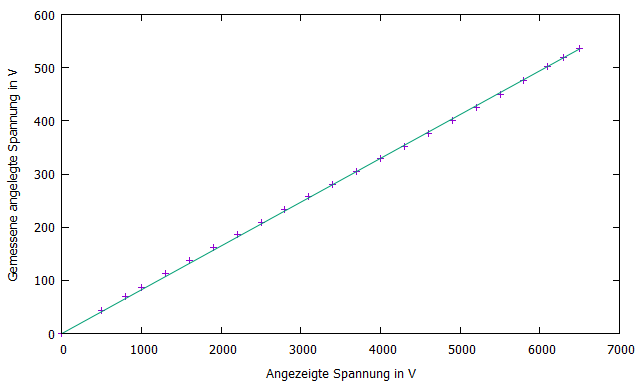
\includegraphics[scale = 0.7]{eichkurve.png}
	\centering
	\caption{Eichkurve der angelegten Wechselspannung an der Ringelektrode; Steigung der Ausgleichsgerade: $0,0824 \pm 0,0002$}
	\label{eichkurve1}
\end{figure}

\section{Versuchsauswertung}

\subsection{Q/m-Werte gefangener Glaskugeln}

Wir haben versucht, geladene Glaskügelchen stabil in der Paul-Falle gefangenzuhalten. Dies ist nur bei zwei Kügelchen für mehr als eine Spannungseinstellung gelungen. Die gemessenen Kugeln können in Tabelle \ref{gefangen} gesehen werden. Zum berechnen des $\frac{Q}{m}$-Verhältnisses der beiden Kugel müssen wir die Spannungen der Deckel- und Bodenelektrode betrachten.

Eine numerische Berechnung des $\vec{E}$-Feldes in der Mitte der Paul-Falle ist aus der Versuchsanleitung vorgegeben als 

\begin{equation}
	E_{Mitte} = \frac{0,798 \cdot (U_{Deckel} - U_{Boden})}{2 z_0}
	\label{emitte1}
\end{equation}

$z_0$ ist der Abstand von der Mitte bis zum Boden/zur Decke der Paul-Falle. Wenn das E-Feld die Gravitationskraft eines Glaskügelchens kompensiert muss gelten

\begin{equation}
	Q E = m g
\end{equation}

Daraus folgt durch Einsetzen von \eqref{emitte1}

\begin{equation}
	\frac{Q}{m} = \frac{2 z_0 g}{0,798 \cdot(U_{Deckel} - U_{Boden})}
	\label{mqformel1}
\end{equation}

 Der Abstand zwischen Boden- und Deckelelektrode ist als $\frac{10}{\sqrt{2}}mm$ gegeben. Somit folgt $z_0 = \frac{5}{\sqrt{2}}mm$.
 
 Der mit \eqref{mqformel1} berechnete Wert von $\frac{Q}{m}$ ist für Kugel Nummer 1 $(4,6 \pm 0,4)*10^{-3} \frac{kg}{C}$. Die Standardabweichung wurde als Fehler genommen. Für Kugel Nummer 2 lässt sich $\frac{Q}{m}$ nicht berechnen, weil Deckel- und Bodenspannung identisch sind. Weil für kleinere Differenzen von $U_{Deckel}$ und $U_{Boden}$ $\frac{Q}{m}$ größer wird, kann man vermuten, dass Kugel Nummer 2 einen großen Wert für $\frac{Q}{m}$ hat. Weil wir nur für eine Kugel den Wert für $\frac{Q}{m}$ bestimmen konnten, ist es uns nicht möglich, Aussagen darüber zu treffen, in welchen Bereichen die Werte für die spezifische Ladung der Glaskügelchen liegen.

\begin{table}[h!]
	\centering
	\begin{tabular}{|l|l|l|l|l|}\hline
		Kugelnummer & $U_{Deckel}$/V ($\pm 1V$)& $U_{Boden}$/V ($\pm 1V$)& $U_{Ring}$/V ($\pm 1V$)& Wechselspannungsfrequenz f/Hz\\\hline
		1 & 158 & 142 & 267 & 101\\
		1 & 161 & 140 & 306 & 101\\
		1 & 160 & 141 & 317 & 101\\
		1 & 161 & 140 & 286 & 101\\
		2 & 150 & 150 & 323 & 101\\
		2 & 150 & 150 & 292 & 101\\\hline
	\end{tabular}
	\caption{Messwerte für in der Paul-Falle gefangene Glaskügelchen}
	\label{gefangen}
\end{table}

\subsection{Stabiler Bereich im a/q-Raum}

Wir betrachten die Werte für a und q, bei denen die Glaskügelchen unserer Messungen stabil waren. a und q lassen sich mit folgenden Formeln berechnen:

\begin{equation}
	a = -8 \frac{Q}{m} \frac{U}{r_o^2 (2 \pi f)^2}
\end{equation}
\begin{equation}
	q = -4 \frac{Q}{m} \frac{V_0}{r_0^2 (2\pi f)^2}
\end{equation}

Der Durchmesser der Ringelektrode ist mit $10mm$ gegeben. Daraus ergibt sich $r_0 = 5mm$.

Für die zweite Kugel war die spezifische Ladung nicht zu berechnen. Deshalb wir nur die stabilen Bereiche der ersten Kugel betrachten. In Tabelle \ref{gefangen2} sind die benötigten gemessenen Werte zur Berechnung von a und q angegeben. Die daraus berechneten Werte sind auch in der Tabelle zu sehen.

\begin{table}[h!]
	\centering
	\begin{tabular}{|l|l|l|l|l|l|}\hline
		Kugelnummer & Gleichspannung U/V ($\pm 2V$) & Wechselspannung $V_0$/V ($\pm 1V$)& f/Hz & a & q\\\hline
		1 & 16 & 267 & 101 & $-0,059 \pm 0,009$ & $-0,49 \pm 0,04$\\
		1 & 21 & 306 & 101 & $-0,077 \pm 0,01$ & $-0,56 \pm 0,05$\\
		1 & 19 & 317 & 101 & $-0.069 \pm 0,009$ & $-0.58 \pm 0,05$\\
		1 & 21 & 286 & 101 & $-0,077 \pm 0,01$ & $-0,52 \pm 0,05$\\
		2 & 0 & 323 & 101 &&\\
		2 & 0 & 292 & 101 &&\\\hline
	\end{tabular}
	\caption{Gemessene Spannungen und berechnete Werte für a und q}
	\label{gefangen2}
\end{table}

\begin{figure}[h]
	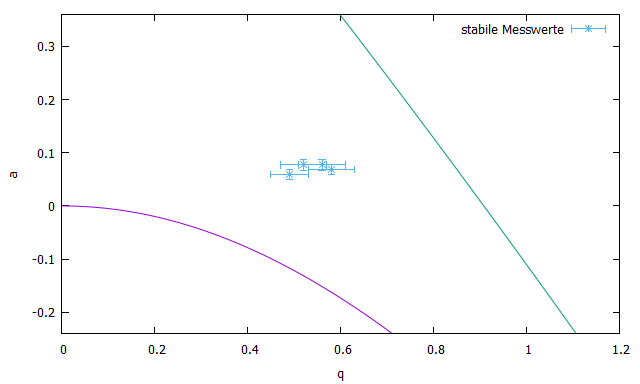
\includegraphics[scale = 0.7]{stabiler_bereich.png}
	\centering
	\caption{Messwerte für stabile Glaskügelchen im Stabilitätsdiagramm}
	\label{stabiler_bereich1}
\end{figure}

\end{document}